\def\name{Two Illustrating Examples}

\begin{frame}{\name{}}
    \textbf{Problem}
    \begin{squarelist}
        \item Quarter five-spot problem with water injection in oil-filled reservoir
        \item Incompressible flow, linear relative permeabilities, equal viscosities
        \item Assume $\log \perm$ is Gaussian with given covariance function $\rightarrow$ 1000 realizations
    \end{squarelist}
    \visible<2->{
        \vspace{0.5em}
        \textbf{Strategy}
        \begin{numlist}
            \item Run MC simulation with 100 samples, compute RMSE $\err^{\mc}$
            \item For layer $0 \dots, L$, run 10 warmup samples to estimate $\cost_\ell$ and $\vara_\ell$
            \item Compute $\nsamp_\ell$ for desired tolerance $\tol \approx \err^{\mc}$, run and compare with MC
        \end{numlist}
    }
\end{frame}

\def\name{Example 1: Smooth Permeability}

\begin{frame}{\name{}}
    \begin{figure}
        \centering
        \only<1>{%
            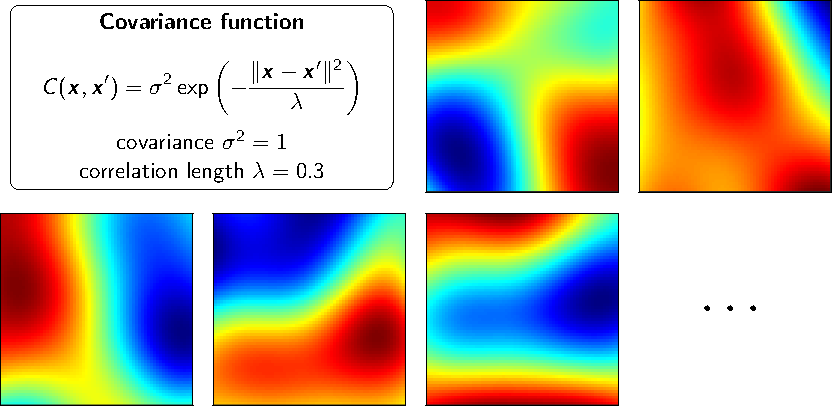
\includegraphics[width = \textwidth]{figures/example-1/perm/ex1-perm.pdf}
        }%
        \only<2>{%
            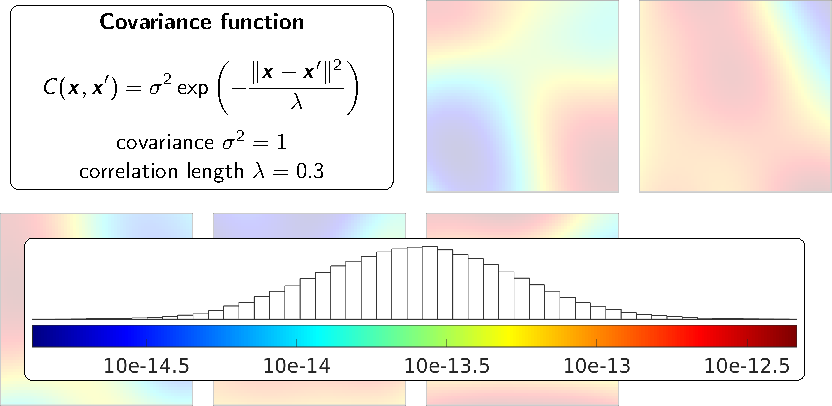
\includegraphics[width = \textwidth]{figures/example-1/perm/ex1-perm-cb.pdf}
        }%
        \only<3>{%
            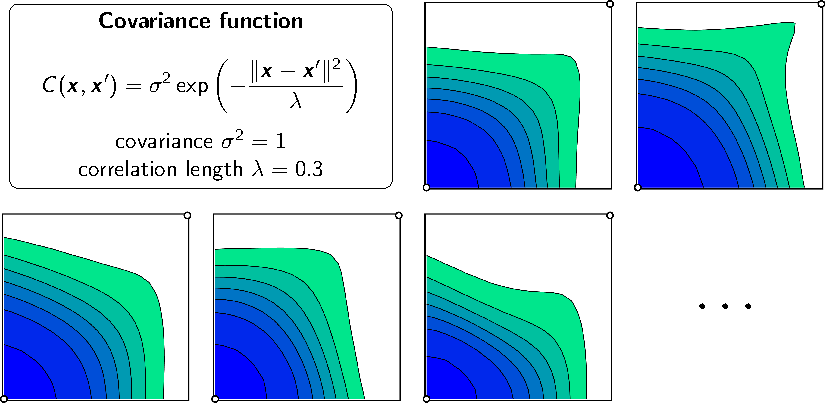
\includegraphics[width = \textwidth]{figures/example-1/sat/ex1-sat.pdf}
        }%
        \only<4>{%
            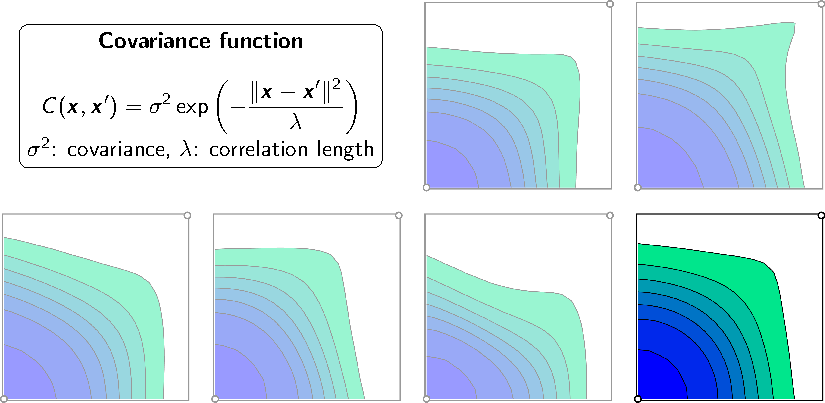
\includegraphics[width = \textwidth]{figures/example-1/sat/ex1-meansat.pdf}
        }%
    \end{figure}
\end{frame}

\begin{frame}{\name{}}
    \begin{figure}
        \centering
        \textbf{Water production rate (m$^3$/day)}
        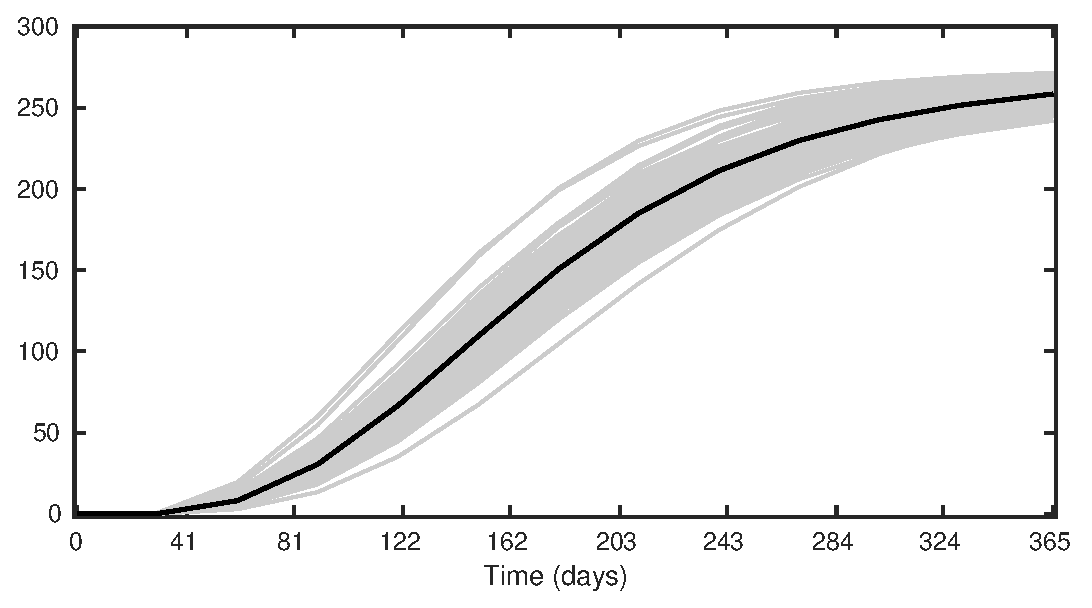
\includegraphics[width = 0.7\textwidth]{figures/example-1/water-rate.eps}
    \end{figure}
    \begin{squarelist}
        \item Monte Carlo simulation with 100 samples: $\err^\mc(q_w) = 1.0\times10^{-2}$
    \end{squarelist}
\end{frame}

\begin{frame}{\name{}}
    \begin{figure}
        \centering
        \only<1>{%
            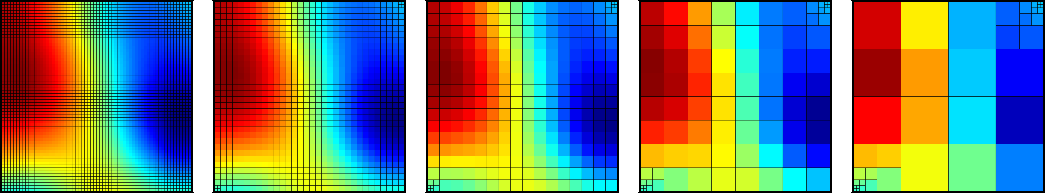
\includegraphics[width = \textwidth]{figures/example-1/permup/ex1-permup.pdf}
        }%
        \only<2>{%
            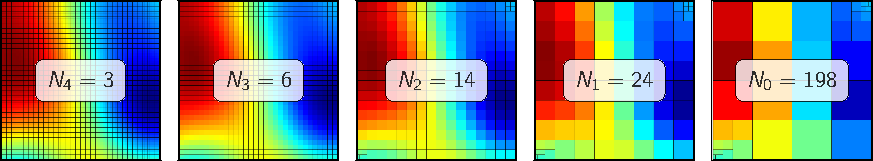
\includegraphics[width = \textwidth]{figures/example-1/permup/ex1-permup-nl.pdf}
        }%
    \end{figure}
    \begin{squarelist}
        \item<1-> Five levels with $\sim$ $4^2$, $8^2$, $16^2$, $32^2$, $64^2$ cells + refinement around wells
        \item<2-> Warmup: Run 10 samples on each level to estimate $\vara_\ell$ and $\cost_\ell$ \\
        $\rightarrow$ used to find optimal $\nsamp_\ell$ for tolerance $\tol = \err^{\mc}$
        \begin{equation*}
            \min\, \sum_{\ell = 0}^\nlev \nsamp_\ell \cost_\ell \quad \text{s.t.} \quad \sum_{\ell = 0}^\nlev\frac{\vara_\ell}{\nsamp_\ell} = \tol^2 \quad \rightarrow \quad \nsamp_\ell = \tol^{-2}\left(\sum_{k = 0}^\nlev \sqrt{\vara_k \cost_k}\right)\sqrt{\frac{\vara_\ell}{\cost_\ell}}
        \end{equation*}
    \end{squarelist}
\end{frame}

\begin{frame}{\name{}}
    \begin{figure}
        \centering
        \textbf{Water production rate (m$^3$/day)}
        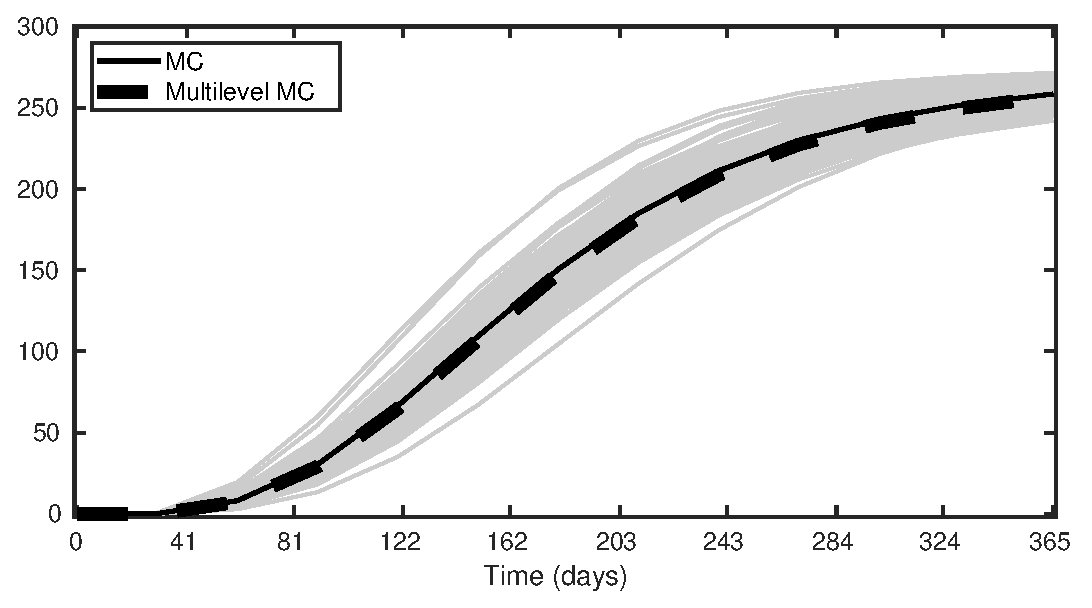
\includegraphics[width = 0.7\textwidth]{figures/example-1/water-rate-ml.eps}
    \end{figure}
    \begin{squarelist}
        \item Multilevel Monte Carlo simulation: $\err^\ml(q_w) = 1.5\times10^{-2}$
    \end{squarelist}
\end{frame}

\begin{frame}{\name{}}
    \begin{figure}
        \centering
        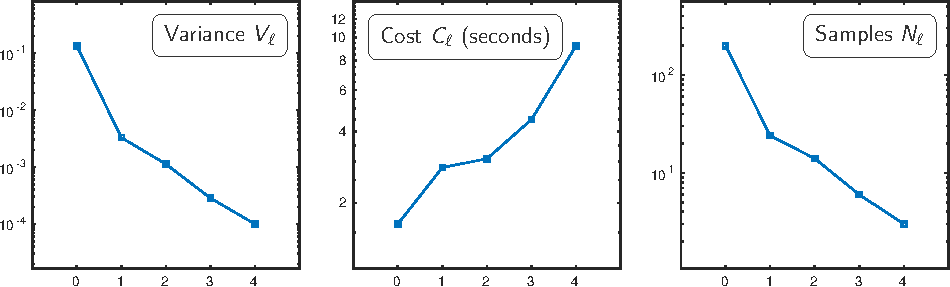
\includegraphics[width = \textwidth]{figures/example-1/statistics/ex1-statistics.pdf}
    \end{figure}
    \begin{squarelist}
        \item<2-> Total cost of Multilevel Monte Carlo: $\sum_\ell \nsamp_\ell \cost_\ell \approx 488$ s
        \item<3-> Total cost of Monte Carlo (assuming $\cost_4 = $ cost of $\un_4 -\un_3$ $\approx$ cost of $\un_4$) $\approx 923$ s\\
        $\rightarrow$ Similar accuracy with about half the cost
    \end{squarelist}
\end{frame}

% nsamples =

%      3
%      6
%     14
%     24
%   198


% c =

%     9.2327
%     4.5050
%     3.0733
%     2.8226
%     1.6266


%% run 2

% nsamples =

%      3
%      7
%     15
%     24
%   132

% c =

%     9.2925
%     4.6800
%     2.9892
%     2.6971
%     1.4028